\subsection{用語の定義}
いくつかの用語を定義する。

\paragraph{確率密度関数 (probability density function: PDF)}
確率変数が連続的な値を取るときその分布を記述する関数のこと。
確率変数を$f(x)$と書くと、次のような性質をもつ。
\begin{itemize}
    \item $f(x) \geq 0$
    \item $\int_{-\infty}^{\infty} f(x)dx = 1$
\end{itemize}
また、確率密度関数は確率変数がある値をとる確率を示すわけではないが、確率変数がある区間に含まれる確率を計算することができる。
確率変数$X$が区間$[a, b]$に含まれる確率は次のように計算できる。
\begin{equation}
    P(a \leq X \leq b) = \int_{a}^{b} f(x)dx
\end{equation}

\paragraph{累積分布関数 (cumulative distribution function: CDF)}
累積分布関数とは、ある確率密度関数$f(x)$に対して、$x$以下の確率を表す関数で次で定義される。。
\begin{equation}
    F(x) = P(X \leq x) = \int_{-\infty}^{x} f(x)dx
\end{equation}

\paragraph{分位数 (quantile)}
分位数は確率変数の値を確率的に分割する点であり、ある確率$p$以下になる確率変数の最大の値と定義される。
分位数は累積分布関数と
\begin{equation}
    F(x) = P(X \leq x) = p
\end{equation}
なる関係にあり、$F(x)$の逆関数である。

これら、標準正規分布におけるPDF, CDF, Quantileの関係を図\ref{fig:pdf-cdf-quantile}に示す。
\begin{figure}
    \centering
    \begin{subfigure}{0.48\columnwidth}
        \centering
        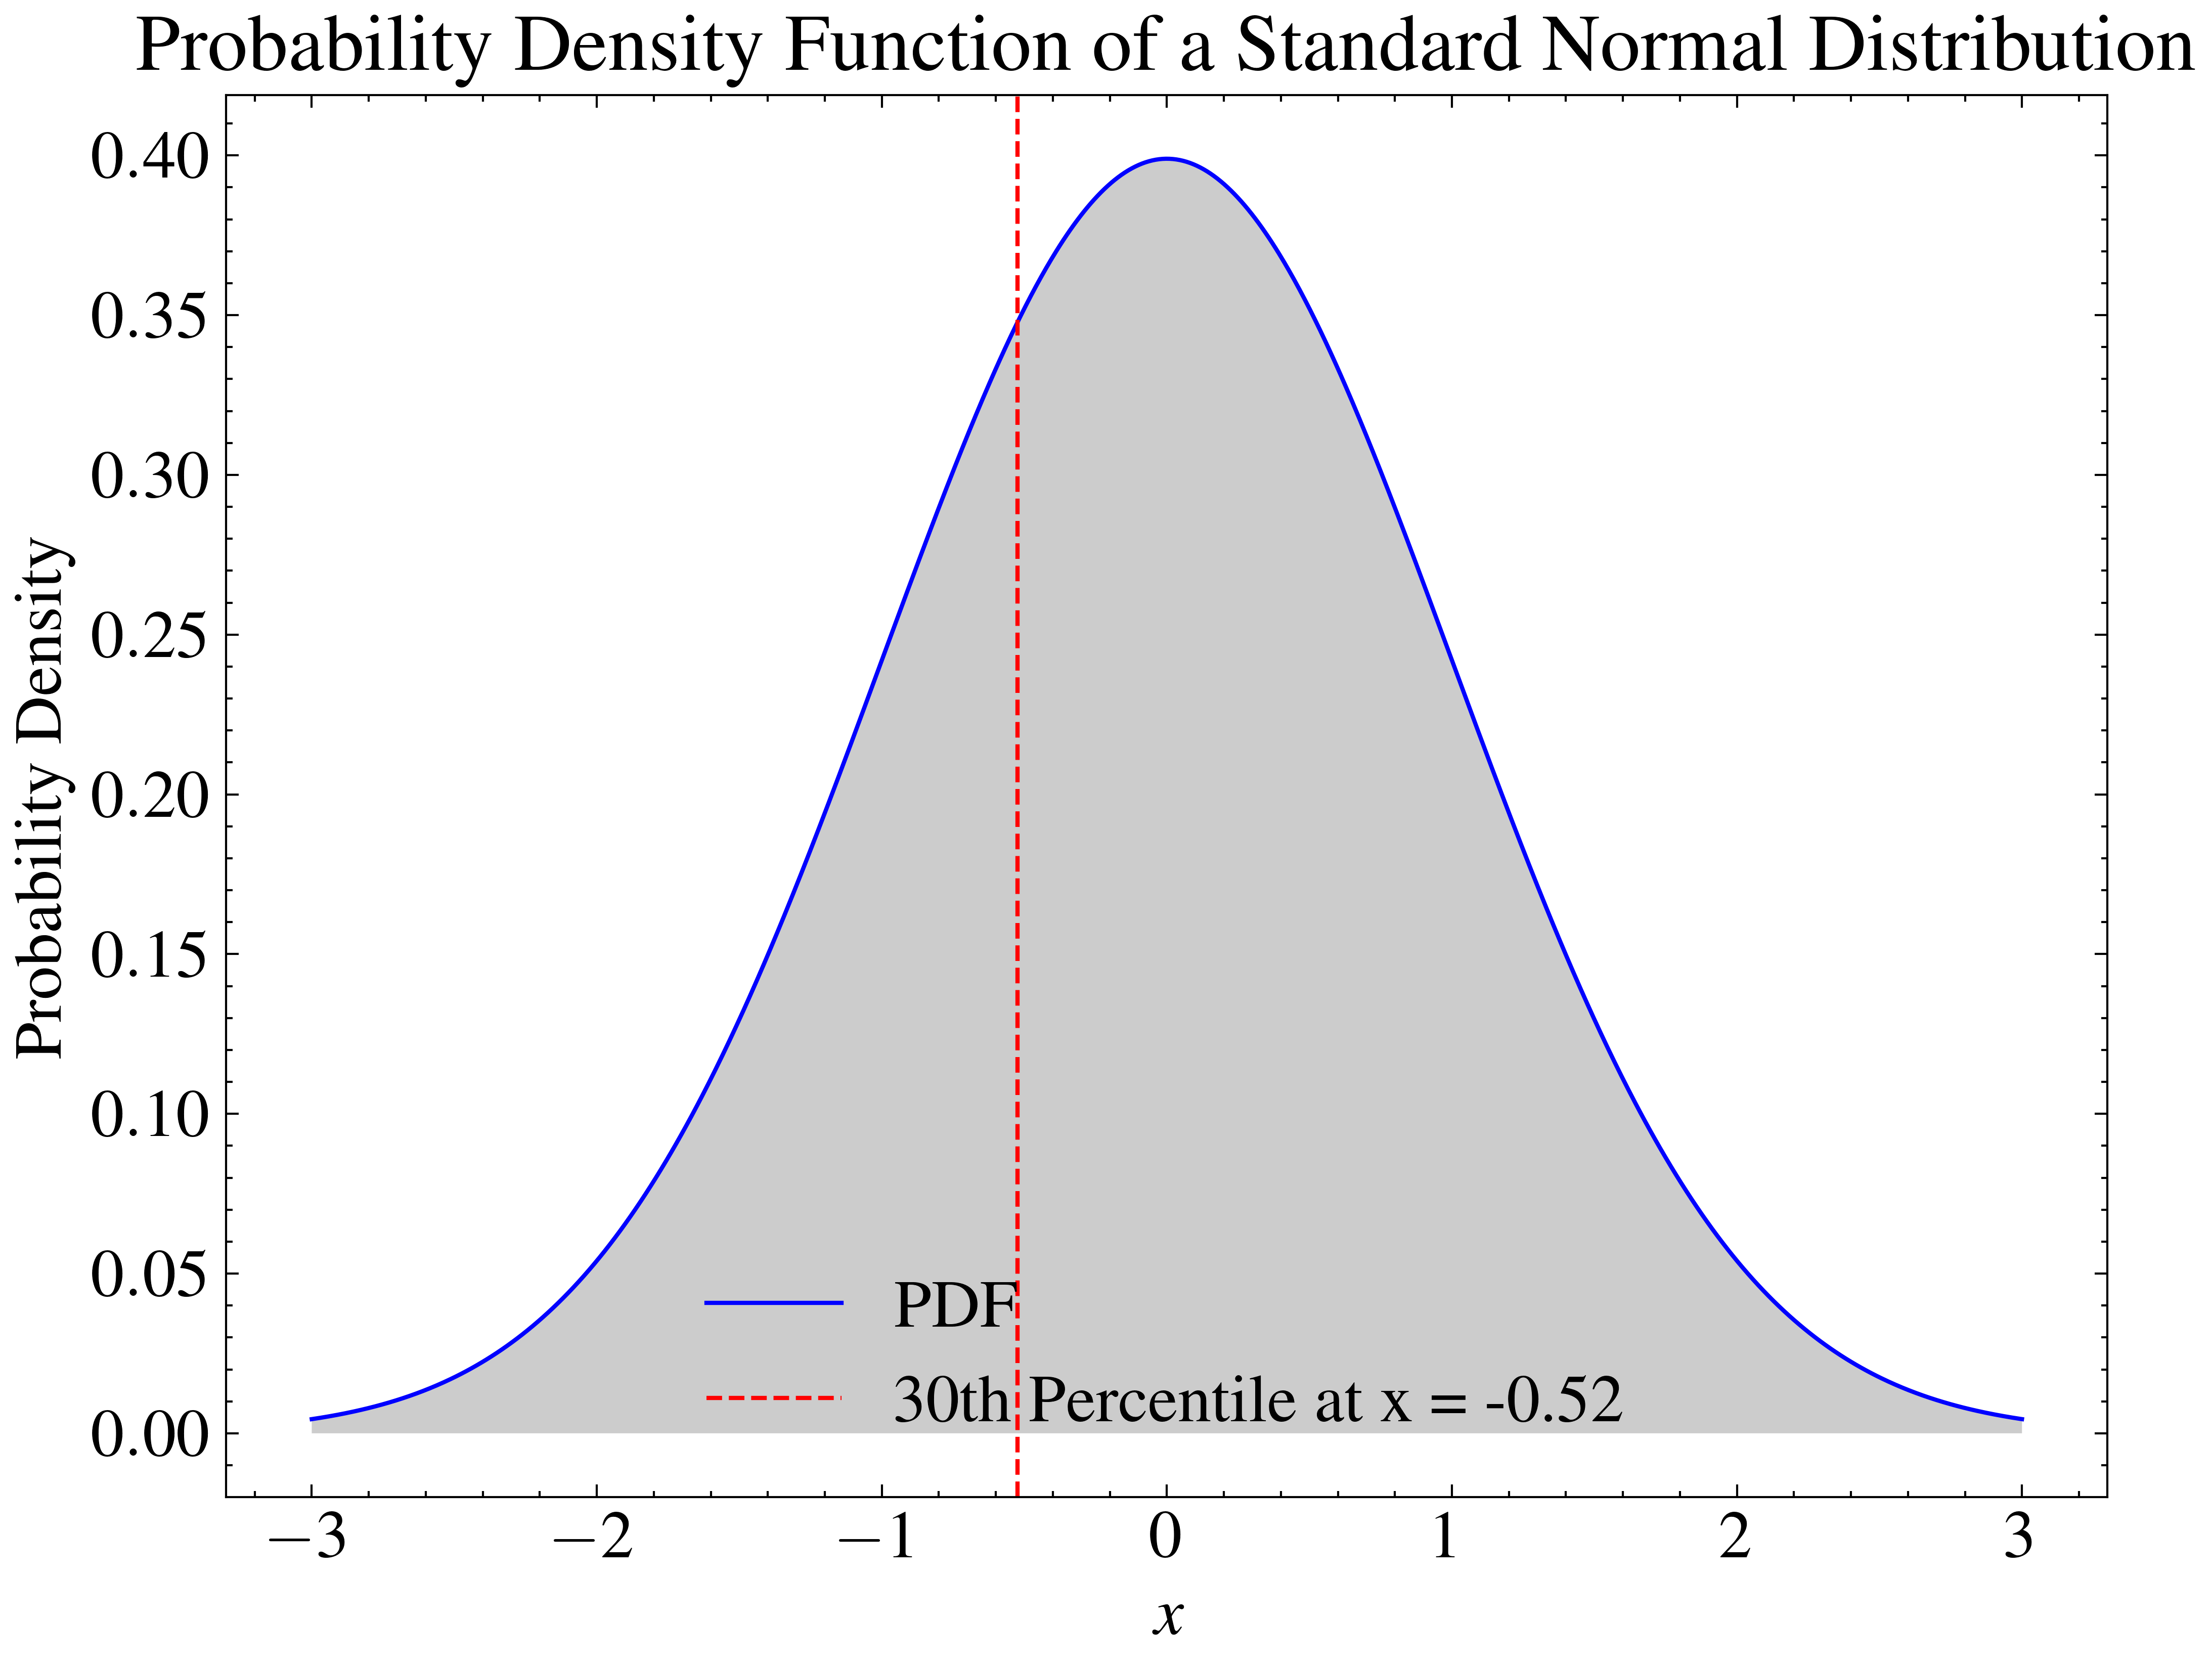
\includegraphics[width=0.8\linewidth]{src/figures/pdf-cdf-quantile/pdf-quantile.png}
        \subcaption{PDF and Quantile}
    \end{subfigure}
    \begin{subfigure}{0.48\columnwidth}
        \centering
        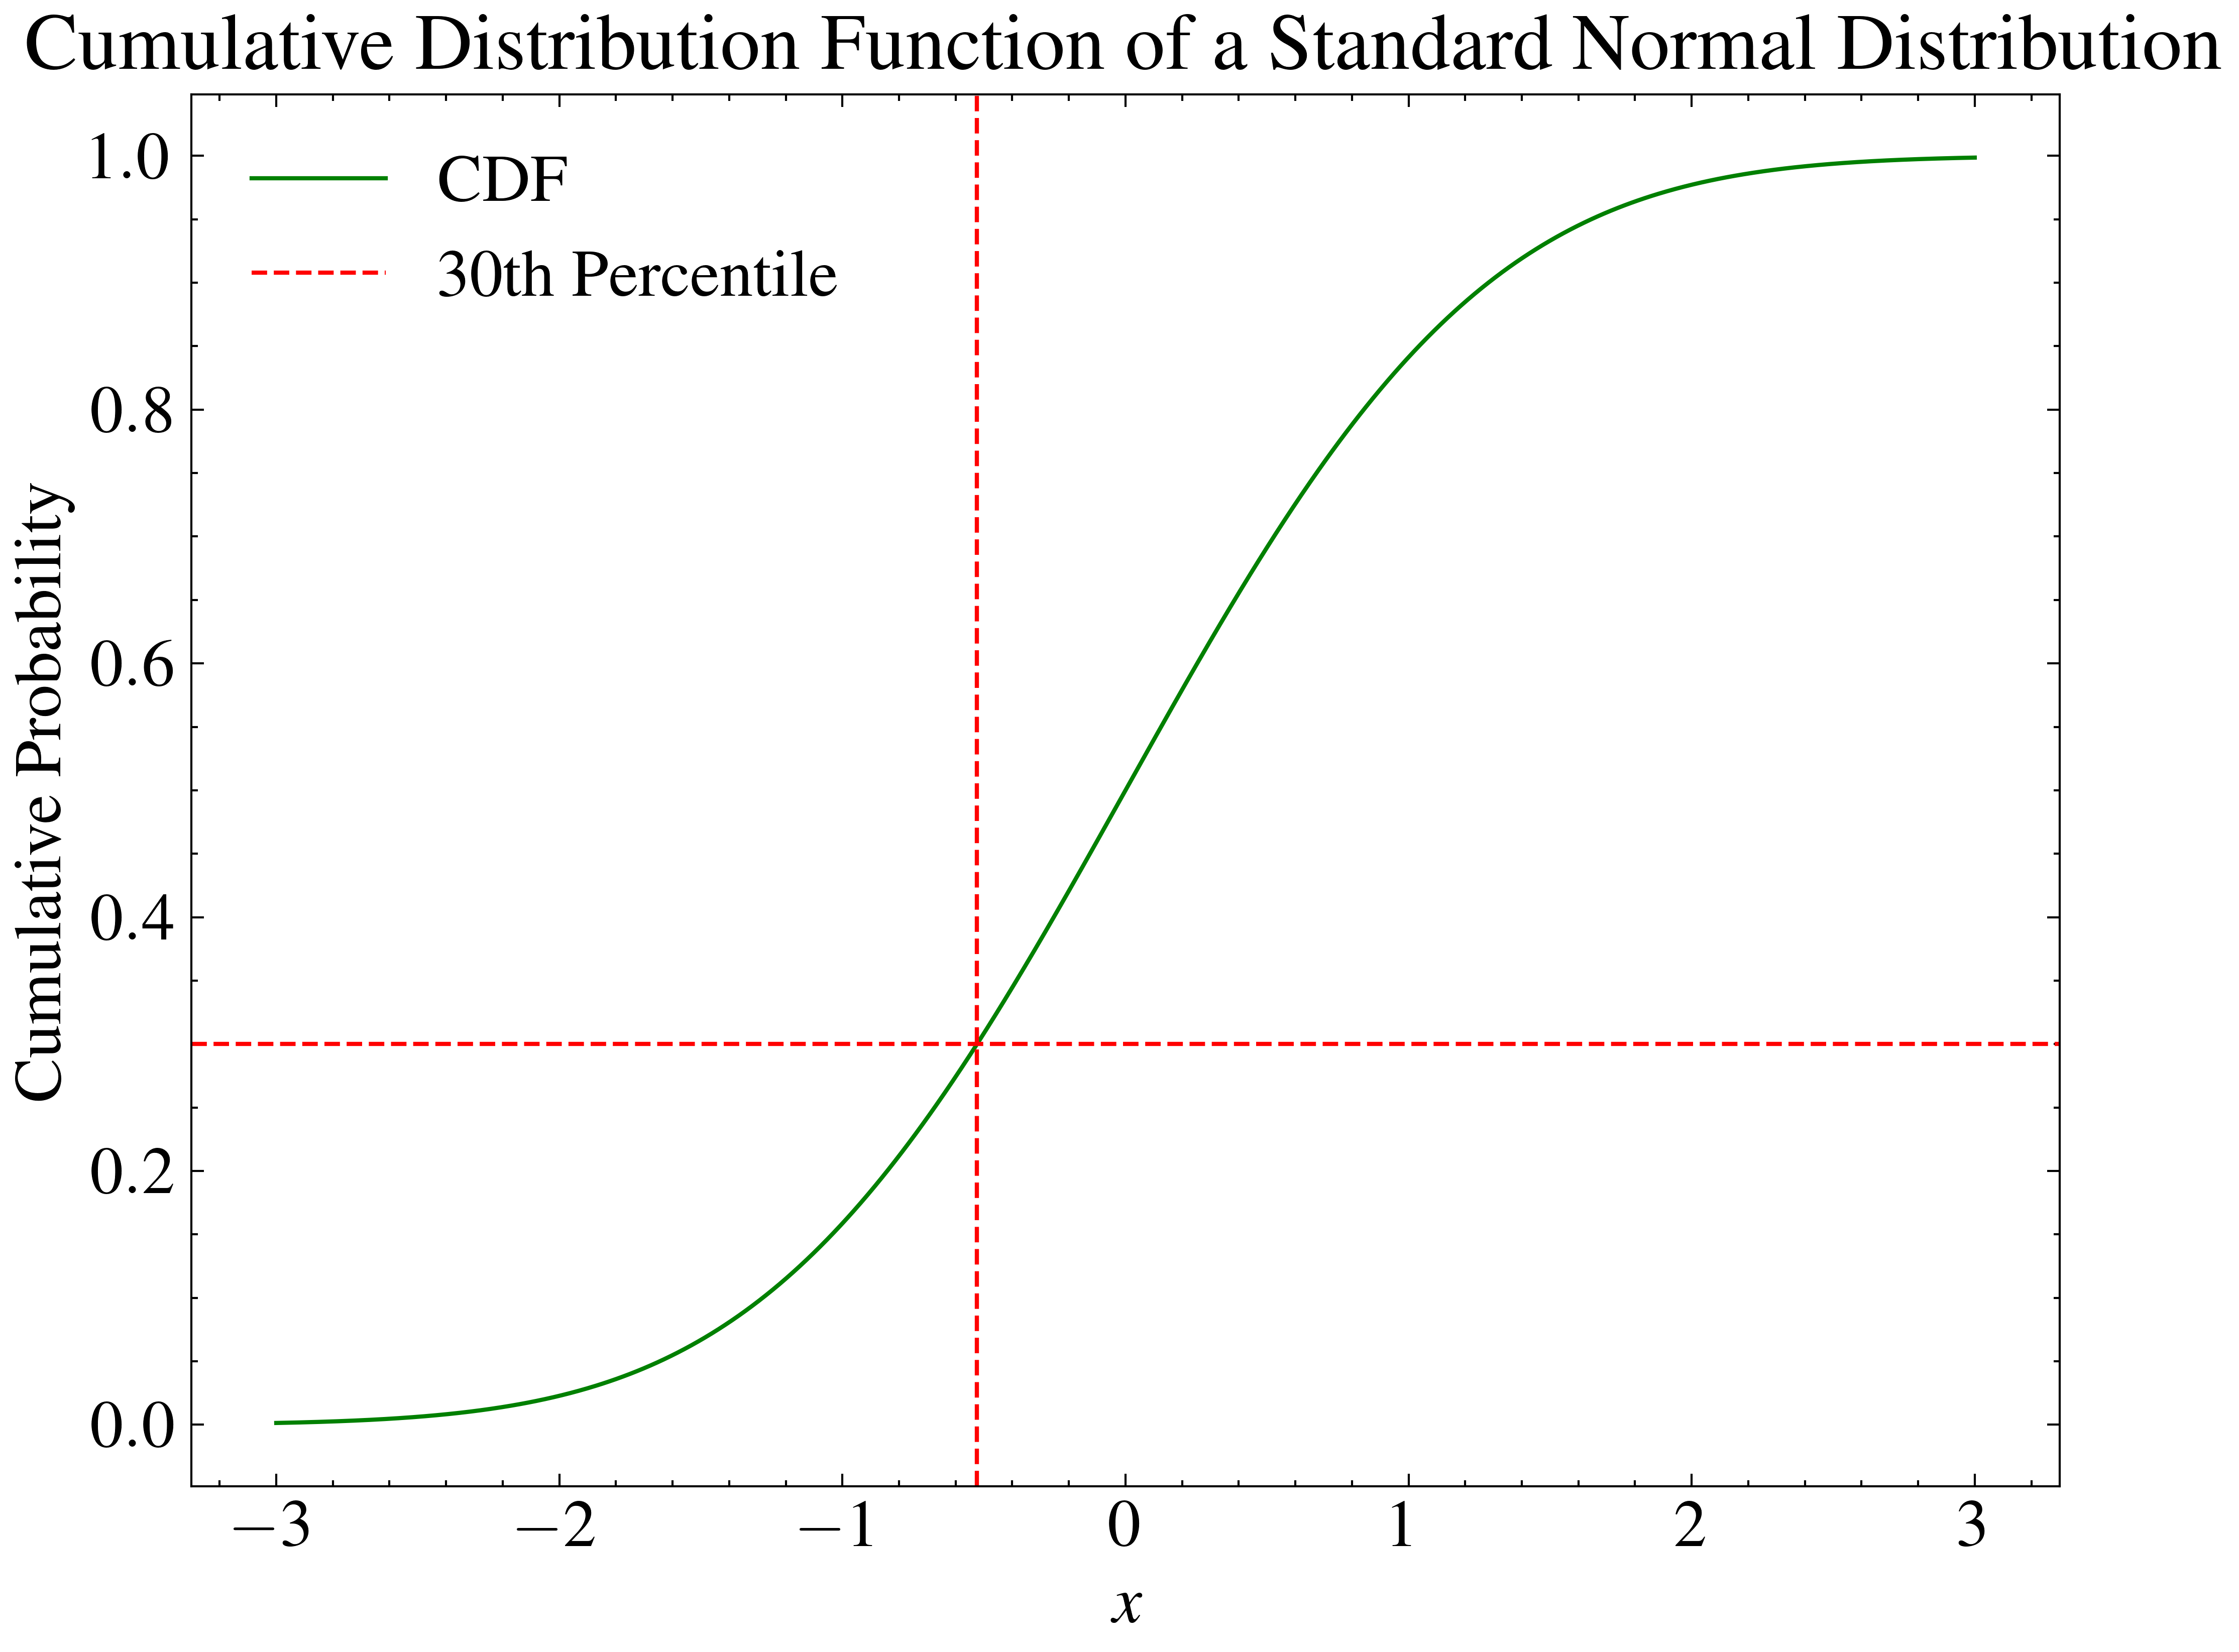
\includegraphics[width=0.8\linewidth]{src/figures/pdf-cdf-quantile/cdf-quantile.png}
        \subcaption{CDF and Quantile}
    \end{subfigure}
    \caption{PDF, CDF and Quantile}\label{fig:pdf-cdf-quantile}
\end{figure}

